\svnInfo $Id$

\section{Bus Design}
\label{sec:protocol}
During normal operation, \bus remains in Bus~Idle~(\ref{sec:protocol-idle}).
A transmission begins with Arbitration~(\ref{sec:protocol-arbitration}), then
Message Transmission~(\ref{sec:protocol-transmission}). The transmitter then
Interrupts~(\ref{sec:protocol-interrupt}) the bus and indicates the complete
message was sent. During the Control~(\ref{sec:protocol-control}) period
acknowledgment is negotiated. After Control, \bus returns to Idle or may
optionally send a response message.

\begin{figure}[h!]
  \figTimingArbitration
\end{figure}

\subsection{Bus~Idle}
\label{sec:protocol-idle}
In \bus Bus~Idle, all lines (clock and data) are high. All member nodes are in
forwarding state and the master node is waiting to begin arbitration.

\subsection{Arbitration}
\label{sec:protocol-arbitration}
To begin arbitration, the bus must be in idle state.

To request to transmit on the bus, a node should pull its {\tt DOUT} line low.
All member nodes remain in forwarding state during arbitration, thus when
their {\tt DIN} line goes low, they are obligated to pull their {\tt DOUT}
line low. The master node, however, does {\bf NOT} pull its {\tt DOUT} line
low in response to its {\tt DIN} line going low. The master node only pulls
its {\tt DOUT} line low when it wishes to transmit on the bus. When the
master node's {\tt DIN} line goes low, it will pull the {\tt CLK} line low
and hold it low for some period $t_{long}$. During {\sc idle} (and thus
arbitration), member nodes must forward the clock signal.

By the end of the period $t_{long}$, the effect of the arbitration is
achieved. A member node is in one of three possible states:
\begin{enumerate}
  \item Clock low, {\tt DIN} high, {\tt DOUT} high -- Lost arbitration
    (didn't participate)
  \item Clock low, {\tt DIN} high, {\tt DOUT} low -- Won arbitration
  \item Clock low, {\tt DIN} low, {\tt DOUT} low -- Lost arbitration
    (either lost, or didn't participate)
\end{enumerate}
The rising edge of clock that follows $t_{long}$ commits the results of
arbitration and all participating member nodes advance their state machines
appropriately.

If the master node wishes to transmit on the bus, all member nodes will be in
the third state. Note this arbitration protocol introduces a {\em
topology-dependent priority}. Firstly, the master node has a greater priority
than any member node as its {\tt DOUT} will propagate around the entire data
loop. The priority of the member nodes is inversely related to their proximity
to the master node in the data loop. That is, the furthest node from the
master node, the node whose {\tt DIN} is connected to the master node's
{\tt DOUT}, has the highest priority of member nodes. The closest node to the
master node, the node whose {\tt DOUT} is connected to the master node's
{\tt DIN}, has the lowest priority.

At the end of $t_{long}$, the master node drives the clock high. The
normal arbitration phase ends on this rising edge. The next two clock edges
allow for a high-priority arbitration. As \bus priority is topology-dependent,
we provide a priority arbitration cycle to allow a low priority member node to
preempt transmissions. This priority mechanism is still topology-dependent,
that is, if Node~1 in Figure~\ref{fig:arbitration} had also attempted to send
a priority message, it would have won that arbitration as well. The priority
arbitration cycle is two clock edges (one clock cycle), the falling edge after
arbitration is for nodes to drive their priority requests onto the bus and the
rising edge is used to latch the results.  During priority arbitration, the
node that won the original arbitration {\bf must not} forward its {\tt DIN} to
{\tt DOUT}. At the end of priority
arbitration, if the original winner did not request a priority message, the
node must sample its {\tt DIN} line. If the line is still low there was no
priority message, if the {\tt DIN} line has gone high, however, the node
has lost priority arbitration and must back off to allow the priority message
requester to transmit.

Whichever node ultimately won arbitration transitions from a forwarding node
to a transmitting node. Nodes that lost arbitration revert to
Forwarding.{\sc Address\_Match}.

\begin{figure}
  \figTimingInterrupt
\end{figure}

\subsection{Message Transmission}
\label{sec:protocol-transmission}
The falling edge after arbitration is defined as ``Begin~Transmission''. On this
edge, the transmitting node should switch its {\tt DOUT} mux from forwarding
{\tt DIN} to the transmit FIFO. Data is expected to be valid and stable during
every subsequent rising clock edge.

The first sequence of bits pushed onto \bus are the {\em address} bits. All
nodes on a \bus should listen until their address:
\begin{itemize}
  \item Matches: Node promotes itself from Forwarding.{\sc address\_match} to
    Receiving.{\sc receive}.
  \item Does Not Match: Node transitions from Forwarding.{\sc address\_match}
    to Forwarding.{\sc Ignore}.
\end{itemize}

There is no protocol-level delineation between address and data bits. The
transmitting node sends address$+$data as a continuous stream of bits (for
details on \bus addressing,
see~\ref{sec:spec-address}~\nameref{sec:spec-address}). Once a transmitter has
sent the complete transmission it Interrupts the bus.

Legal transmissions on \bus must be byte-aligned
(\ref{sec:spec-granularity}~\nameref{sec:spec-granularity}). The requirement
allows receiving nodes such as node~1 and node~3 in Figure~\ref{fig:interrupt}
to disambiguate the significance of the last two bits received. A legal
transmission will end cleanly on a byte boundary if the node topologically
follows the transmitter (e.g.~node~3) or will end on a byte+2-bit boundary if
the node topologically precedes the transmitter (e.g.~node~1).

\subsection{Interrupt}
\label{sec:protocol-interrupt}
During normal operation, Interrupt is only permitted after the first 32~bits
of data have been transmitted
(\ref{sec:spec-interrupt}~\nameref{sec:spec-interrupt}). The Interrupt
mechanism, however, is also the \bus reset mechanism, and as such member node
interrupt detectors {\bf must} always be active whenever a node is not Idle.

A \bus interrupt is defined as a series of pulses on the data line while the
clock line remains high. After $N$~pulses where $N \ge 3$, a node enters
Interrupt\footnote{
  While two pulses is sufficient to distinguish an Interrupt from normal data
  transmission, three pulses provides protection against spurious entry to
  Interrupt from a glitch on data lines.}.
Edges on the data line while the clock is low are ignored. This permits
potentially racy changes of {\tt DOUT} drivers to safely change on the falling
edge of the clock without potentially introducing spurious interrupts.

The first rising clock edge after Interrupt is defined as ``Begin~Control''.
The next two clock edges define the control bits.

\subsubsection{Nesting Interrupts}
In normal operation, interrupts are not permitted to ``nest'', that is, the
bus may not be interrupted while the control bits are being sent. If an
Interrupt sequence occurs during an existing Interrupt (which may only occur
if the bus is being ``rescued'' from some erroneous state), the new interrupt
{\bf must} present control bits {\tt 00}. Any operations requested from the
previous Interrupt state are aborted and the net Interrupt result is
{\tt 00}~(General~Error).

\subsection{Control Bits}
\label{sec:protocol-control}

\begin{figure}
  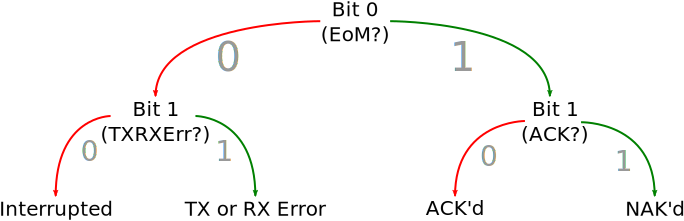
\includegraphics[width=\linewidth]{img/control_bits}
  \caption{After an Interrupt, two control bits follow. The first bit is
    always set by the interrupter and indicates whether the Interrupt was to
    signal the end of message (EoM). If the EoM bit is high, the receiving
    node is responsible for driving the second bit to acknowledge the message.
    If the EoM bit is low, the interrupter is responsible for driving the
    second bit. The TX/RX~Error (TRE) bit is set when a transmitting or
    receiving node encounters an error.
  }
  \label{fig:control-bits}
\end{figure}

The two bits after an Interrupt are defined as Control~Bits.
Figure~\ref{fig:control-bits} is a flowchart indicating the semantic meaning
of the control bits and the resulting state. The first control bit is
unconditionally driven by the interrupting node. If a transmitting node has
interrupted to indicate the end of transmission, it will put a {\tt 1} on the
bus for the first control bit. In all other cases the interrupter must drive
{\tt 0} for the first control bit.

If the first control bit was {\tt 1} then the addressed receiver is
responsible for driving the second control bit. If the transmission was sent
to the broadcast address~(\ref{sec:control-broadcast}), all nodes---excluding
the transmitter which forwards---should drive the second control bit low to
acknowledge. The semantic provided to the transmitter of a broadcast message
then is either (1) no nodes received the message or (0) {\em at least} one
node received the message.

If instead the first control bit was {\tt 0} then the interrupter is
responsible for driving the second control bit. If the interrupter is the
transmitter or receiver {\bf and} the issue is related to the current
transmission (e.g. receiver buffer overflow) then the second bit should be set
high. If the purpose of the interruption is unrelated to the current
transmission (e.g. an external, high-priority, time-critical message) then the
second bit should be set low.

Unless the interruption carries a specific meaning as outlined in this
section, the {\sc 00: Interrupted} state should be used for general or
unclassified interruptions as it carriers the least semantic meaning

\subsection{Return to Idle}
\label{sec:protocol-return-idle}
After latching the final Control~Bit (time~20 in
Figure~\ref{fig:interrupt}), one final edge (time~22) is generated to formally
enter {\sc idle}. If, however, the data line is low at this edge, then it
shall be considered the start of a new arbitration cycle instead. The master
node will pull the clock low again in response and begin waiting for
$t_{long}$.

By providing this edge, \bus enables member nodes with absolutely no sense of
time the ability to receive, react to, and respond to messages (albeit with
tight timing constraints).

\begin{quote}
\textit{M3 Implementation Note:} (Referring to
Figure~\ref{fig:interrupt}) A broadcast sleep message cannot be considered a
sleep until time~18 when the transmitter asserts that all the sent bits were
desired to be sent. This leaves edges at time~20 and time~22 as the required
two edges to power gate the layer.

This could be complicated, however, if a node elects (for some reason) to send
a response to the broadcast sleep message. The sleep controller will still
have four edges (Arbitration, Priority~Drive, Priority~Latch,
Begin~Transmission) to wake its bus controller, but the timing between arming
its {\tt CLK\_IN} fall detector and the master node pulling {\tt CLK\_IN} low
in response could cause the sleep controller to miss wakeup.
\end{quote}
